
\section{Example: Modeling the Greenland ice sheet (EISMINT-Greenland)}\label{sec:eismint-greenland} \index{PISM!running the EISMINT-Greenland intercomparison}\index{Greenland ice sheet}\index{EISMINT!intercomparison of Greenland models} 
\optsection{EISMINT-Greenland}

In this section we give an extended example of how to use PISM to model the Greenland ice sheet.  We use older data from the 1990s ice sheet modelling intercomparison EISMINT-Greenland \cite{HuybrechtsEISMINT,RitzEISMINT}, but it is an excellent tutorial example.

The data are freely available at
\medskip

\centerline{\protect{\textbf{\url{http://homepages.vub.ac.be/~phuybrec/eismint/greenland.html}}}}
\medskip

\noindent The snow-fall accumulation map, ablation parameterization, surface temperature formula, surface elevation, and bedrock elevation maps are essentially as in the 1991 papers \cite{Letreguillyetal1991,OhmuraReeh}.  In the ``forced climate'' CCL3 run, described below, the modeled ice sheet is sees changes in surface temperature from the GRIP core \cite{Dansgaardetal1993} and sea level changes from SPECMAP \cite{Imbrieetal1984}.

Substantial developments have occurred in modeling the Greenland ice sheet since the EISMINT-Greenland intercomparison.  For example, the relation between a Greenland ice sheet flow model, Earth deformation under ice sheet loads, and the reconstruction of global ice loading is analyzed in \cite{TarasovPeltier}.  A parameter-sensitivity study of a EISMINT-Greenland-type ice sheet model is described in \cite{RitzFabreLetreguilly}.  The response of Greenland ice sheet models to climate warming is addressed in \cite{HuybrechtsdeWolde,Huybrechts02, Greve00}, among other references.

The rest of this section is a step-by-step PISM tutorial.  The details can be typed in by hand, or the user can invoke the bash scripts \verb|preprocess.sh|, \verb|bootstrap.sh|, \verb|ssl2.sh|, and \verb|ccl3.sh| in the directory \verb|examples/eisgreen|.  These scripts execute the commands in the next four subsections, respectively.

\subsubsection*{Obtaining and pre-processing the EISMINT-Greenland data}  We use two Python scripts to convert the EISMINT-Greenland data.  The data is in the form of several ASCII text files, so we convert them into NetCDF files usable by PISM.  The Python libraries \href{http://numpy.scipy.org/}{\texttt{numpy}} and \href{http://code.google.com/p/netcdf4-python/}{\texttt{netcdf4-python}} must be present for the scripts to work.

First, \verb|cd examples/eisgreen/| from the PISM directory, and download these text (ASCII) files from the EISMINT-Greenland web site above: 

\verb|grid20-EISMINT,  suaq20-EISMINT,  specmap.017,  sum89-92-ss09-50yr.stp|

\noindent (This is done by \verb|preprocess.sh| using \verb|wget|.) Once all four files have been downloaded, run

\verb|$ ./eisgreen.py|

\noindent The NetCDF file \verb|eis_green20.nc| will be created from the data in \verb|grid20-EISMINT| and \verb|suaq20-EISMINT|.  It contains variables for the gridded latitude (\verb|lat|), longitude (\verb|lon|), surface altitude (``\verb|usurf|'' for \emph{u}pper \emph{surf}ace elevation), ice thickness (\verb|thk|), bedrock altitude (\verb|topg|), and snow precipitation rate (\verb|snowprecip|; in ice-equivalent thickness units).  These values can be viewed graphically with \verb|ncview|.  The metadata for these variables (the NetCDF ``header'') can be viewed by

\verb|ncdump -h eis_green20.nc|

The bed elevation \verb|topg| in the original data (\verb|suaq20-EISMINT|) effectively contains missing values.  These are locations where \verb|topg| is \emph{exactly} $0.0$, presumably because in these locations the observed bed elevation was not measured or the measured value was not trusted.  We think these are deep fjords locations, mostly.  Also the topography of Ellesmere island is replaced by out of range negative values.  When viewing \verb|eis_green20.nc| with \verb|ncview|, these values show as white spots.  

If these missing values were to be left in the NetCDF handed to PISM then the resulting (very) rough bed elevation map would make reasonable ice flow results difficult.  We therefore smoothly fill the holes in the bed elevations.  This is done with another script named \verb|fill_missing.py|:\footnote{\texttt{fill_missing.py} is a general tool for smoothly filling patches of missing values in variables in NetCDF files.  It looks for attributes defining missing values and then fills in specified variables essentially by averaging the neighboring non-missing values.  It is found in directory \texttt{pism/util/}, it requires \href{http://code.google.com/p/netcdf4-python/}{\texttt{netcdf4-python}}, and it is documented in subsection \ref{subsect:scripts}.}:

\verb|$ fill_missing.py -f eis_green20.nc -v topg -o eis_green_smoothed.nc|

\begin{figure}[ht]
\centering
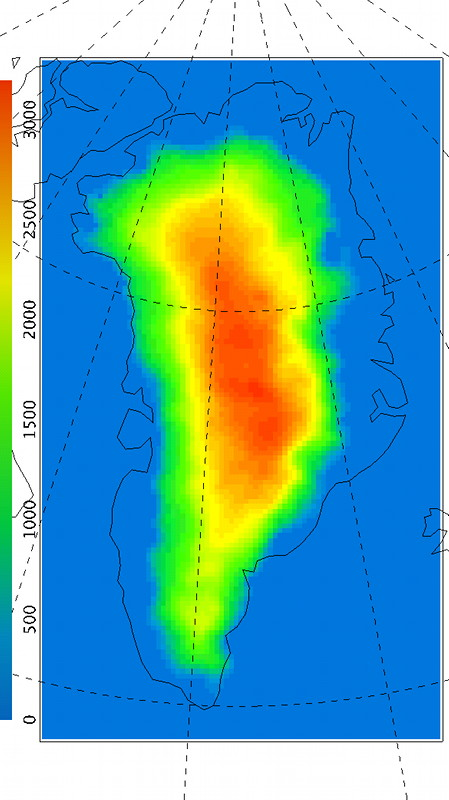
\includegraphics[width=2.4in,keepaspectratio=true]{EISgreen-thick}\quad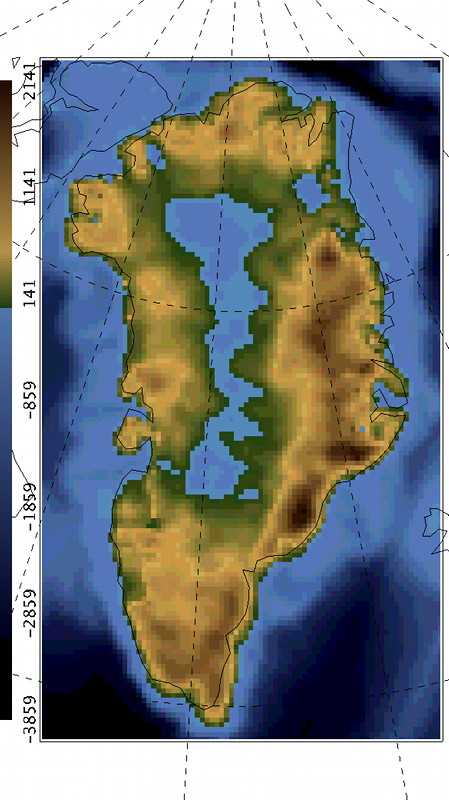
\includegraphics[width=2.4in,keepaspectratio=true]{EISgreen-bed}
\caption{Views of the thickness (left) and smoothed bed elevation (right) for EISMINT-Greenland.  The coastal topography around several fjords has been smoothed.}
\label{fig:greendata}
\end{figure}

Next we use a script which converts the time-series data files \texttt{specmap.017} and \texttt{sum89-92-ss09-50yr.stp} to PISM-readable NetCDF form:

\verb|$ ./eiscore.py|

\noindent Two NetCDF files with one-dimensional time series data are created, namely \verb|grip_dT.nc| and \verb|specmap_dSL.nc|.  In the paleoclimate run ``CCL3'' below, the executable \verb|pgrn| will be called with options \verb|-dTforcing| and \verb|-dSLforcing| on these two \verb|.nc| files, respectively.  Thus PISM will read the GRIP data \cite{Dansgaardetal1993} for the surface temperature forcing and the SPECMAP data \cite{Imbrieetal1984} for sea level forcing.  Figure \ref{fig:gripDeltaT} shows the GRIP temperature offsets.

\begin{figure}[ht]
\centering
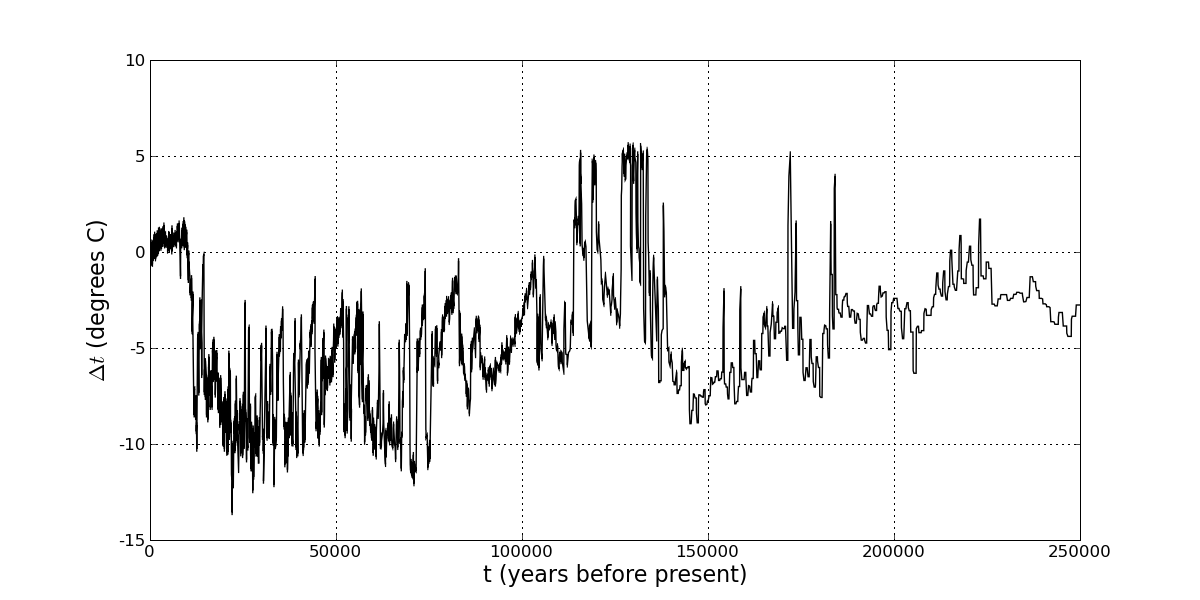
\includegraphics[width=5.6in,keepaspectratio=true]{gripDeltaT}
\caption{Change in temperature from present, from the GRIP core \cite{JohnsenetalGRIP}.}
\label{fig:gripDeltaT}
\end{figure}


\subsubsection*{Bootstrapping}  \label{sect:green-bootstrapping}  Once the EISMINT Greenland data is obtained and converted to NetCDF, as above, ``bootstrapping'' can begin.  By ``bootstrapping'' we mean the creation, by heuristics and simplified models, of the full initial conditions needed for the continuum model.  \footnote{The continuum model is the differential equations describing ice flow inside PISM.  See section \ref{sect:boot} for more on ``bootstrapping''.}

We do a one model year run using option \verb|-boot_from| to ``bootstrap'' from file \verb|eis_green_smoothed.nc|.  The executable ``\verb|pgrn|'' is special to EISMINT-Greenland:\index{pgrn}
\begin{verbatim}
$ pgrn -boot_from eis_green_smoothed.nc \
       -Mx 83 -My 141 -Lz 4000 -Mz 51 -Lbz 2000 \
       -skip 1 -y 1 -o green20km_y1.nc
\end{verbatim}
\noindent The run takes only a few seconds of real time on any machine.  Tables \ref{bootstrapEISgreen} and \ref{bootCONTINUED} show the entire PISM output at the terminal.

\begin{table}
\centering
\scriptsize
\begin{quote}
\begin{verbatim}
PGRN revision 797M trunk (PISM EISMINT-Greenland mode)
  time dimension was not found; setting current year to t = 0.0 years
  setting flags equivalent to '-e 3 -ocean_kill'; user options may override ...
  initializing atmospheric climate coupler with a snow process model ...
    reading mean annual ice-equivalent snow precipitation rate 'snowprecip'
      from eis_green_smoothed.nc ... 
  FOUND  snowprecip/ mean annual ice-equivalent snow precipitation rate          
                   \ min,max =     0.030,    2.820 (m year-1)
    using default snow-surface temperature parameterization
    attempting to read ice surface temperature (energy conservation boundary values) 'artm'
      from eis_green_smoothed.nc ...
  absent artm      / ice temperature at ice surface but below firn processes     
                   \ not found; continuing without setting it
  special climate coupler for EISMINT-Greenland
    -- non-default snow and ice surface temperature parameterizations
    -- non-default interpretation of PDD factors
    -- can add greenhouse warming if -gwl3 chosen
bootstrapping by PISM default method from file eis_green_smoothed.nc
  rescaling computational box for ice from -boot_from file and
    user options to dimensions:
    [-1400.00 km, 1400.00 km] x [-820.00 km, 820.00 km] x [0 m, 4000.00 m]
  WARNING: surface elevation 'usurf' found; IGNORING IT!
  reading 2D model state variables by regridding ...
  FOUND  lon       / standard_name=longitude                          
                   \ min,max =   -94.194,   12.889 (degree_east)
  FOUND  lat       / standard_name=latitude         
                   \ min,max =    58.275,   84.458 (degree_north)
  FOUND  thk       / standard_name=land_ice_thickness                              
                   \ min,max =     0.000, 3200.000 (m)
  FOUND  topg      / standard_name=bedrock_altitude                  
                   \ min,max = -3859.000, 2151.000 (m)
  absent bwat      / effective thickness of subglacial melt water                
                   \ not found; using default constant    0.00 (m)
  absent tillphi   / friction angle for till under grounded ice sheet            
                   \ not found; using default constant   15.00 (degrees)
  absent bheatflx  / upward geothermal flux at bedrock surface                   
                   \ not found; using default constant   50.00 (mW m-2)
  absent dbdt      / bedrock uplift rate                                         
                   \ not found; using default constant    0.00 (m year-1)
  determining surface elevation by  usurf = topg + thk  where grounded
    and by floatation crit  usurf = (1-rho_i/rho_w) thk  where floating
  preliminary determination of mask for grounded/floating and sheet/dragging
    option -ocean_kill seen: floating ice mask=3; ice free ocean mask=7
  filling in ice and bedrock temperatures using surface temperatures and quartic guess
done reading eis_green_smoothed.nc; bootstrapping done
computational box: 2800.00 km x 1640.00 km x (4000.00 m + 2000.00 m bedrock)
horizontal grid cell dimensions: 20.00 km x 20.00 km
  vertical grid spacing in ice: uneven, 51 levels, 21.200 m < dz < 138.800 m
  vertical grid spacing in bedrock: uneven, 17 levels, 21.200 m < dz < 228.800 m
\end{verbatim}
\end{quote}
\normalsize
\bigskip

\caption{Output of bootstrapping command.  Continues in Table \ref{bootCONTINUED}.}
\label{bootstrapEISgreen}
\end{table}

\begin{table}
\centering
\scriptsize
\begin{quote}
\begin{verbatim}
P         YEAR:     ivol   iarea    meltf     thick0     temp0
U        years 10^6_km^3 10^6_km^2 (none)          m         K
S      0.00000:  2.82500  1.6708   0.2071   3042.000  270.5156
 $$ SIA        vath 0d  +0.18294
S      0.18294:  2.82513  2.1068   0.1665   3041.887  270.5156
 $$ SIA        vath 0d  +0.23543
S      0.41837:  2.82480  1.6704   0.2079   3041.702  270.5157
 $$ SIA        vath 0d  +0.26969
S      0.68806:  2.82498  2.0444   0.1708   3041.457  270.5159
 $$ SIA        vath 0d  +0.29958
S      0.98765:  2.82522  2.2280   0.1682   3041.175  270.5161
 $$ SIA        vath 0e  +0.01235
S      1.00000:  2.82523  2.2300   0.1690   3041.164  270.5163
done with run ... 
Writing model state to file `green20km_y1.nc'
\end{verbatim}
\end{quote}
\normalsize
\bigskip

\caption{Continuation of Table \ref{bootstrapEISgreen}.}
\label{bootCONTINUED}
\end{table}

What has happened?  As noted, \emph{all} real ice sheet data fails to contain certain variables necessary to initialize an ice sheet model, in the sense of complete initial values for time-dependent partial differential equations.  For instance, the data and the observation-based parameterizations do not include the temperature of the ice anywhere but at the surface.  The data do not include the amount of water stored at the ice/bedrock interface.  And so on.  These are not omissions from the data sets but rather inevitable facts; one cannot observe ice sheets as fluids very well.  Necessarily, therefore, PISM fills in the unknown initial conditions based on some default guesses, as indicated by the messages in Table \ref{bootstrapEISgreen}.

Note that EISMINT-Greenland specifies an 83 by 141 point grid, but you may use other numbers for \verb|-Mx| and \verb|-My| if desired.  In such cases the data will be linearly interpolated onto your grid.  Larger values will produce slower runs.

The option \verb|-boot_from| stands for ``bootstrap from''.  A different option \verb|-i|, for ``input file'', is used for a file which has full initial conditions.  In practice, \verb|-i| is only used with a NetCDF file which was previously saved by PISM.  That is, \verb|-i| is used to continue a run from a saved state.

Note the choice of the height of the computational box (``\verb|-Lz 4000|''), of the number of vertical levels (``\verb|-Mz 51|'' for levels in ice and ``\verb|-Mbz 51|'' for levels in bedrock). The messages to standard out show that the vertical spacing is about 20 m near the base and more than 130 m at the top of the computational box (where it matters less).

We see the report that bootstrapping has applied an interpolation scheme to the surface temperatures and geothermal fluxes to estimate preliminary temperatures within the ice.  It is based on a heuristic for the amount of downward flow in a column.  Thus bootstrapping quickly creates a temperature field at depth, but it is not a field in equilibrium with the flow.  (That's coming \dots)

The bootstrapping mode also fills in several default values.  For instance, the variables \verb|bwat| (effective thickness of basal water), \verb|tillphi| (till friction angle), \verb|bheatflx| (geothermal flux), and \verb|dbdt| (bed uplift rate) were not found in the input file.   (They would be present in a saved PISM model state and they are part of the ``full initial conditions'' referred to earlier.)  Also, note that the data had redundant surface elevation values in the sense that PISM bootstrapping includes the computation ``\verb|usurf = topg + thk|'' of the surface elevation from the ice thickness and the bed elevation.

In addition to the default bootstrapping actions there are additional settings special to EISMINT-Greenland.  For instance, because there is no EISMINT-Greenland gridded data set for surface temperature \cite{RitzEISMINT}.  Instead there is a formula (parameterization) which determines the temperature as a function of latitude and surface elevation.  The code behind \verb|pgrn| knows this formula and uses it.  Also the prescribed constant value for geothermal flux is set.  Finally, by default the option \verb|-ocean_kill| is set internally in \verb|pgrn|.  This forces all floating ice to immediately calve off (i.e.~to have thickness zero).

As suggested a few paragraphs back, it is helpful to do a better job of filling in the temperatures within the ice.  One way to do this is to have the temperature field and velocity field co-evolve according to the thermomechanical flow model while holding the upper ice surface stationary.  This is a continuation of ``bootstrapping''.  The effect is to create a temperature field which is approximately stationary with respect to advection and conduction.\footnote{The resulting temperature field is not a fully physical temperature field, however, because it comes from a steadiness assumption about the geometry of the ice sheet.  Said another way, it is a temperature field in equilibrium with a velocity field for which the surface kinematical equation \cite{Fowler} is \emph{not} satisfied.}  We create this temperature field by running for 25000 years\footnote{In fact a longer run is reasonable.  The exponential time constant for decay of the thermomechanically-coupled system toward equilibrium is on the order of 100k years.  But the goal is merely to get to a state which is reasonable for starting a complete steady-state run.} with non-evolving surface.  The option \verb|-no_mass| turns off the map-plane mass continuity scheme, and thus any evolution of the surface.

\begin{verbatim}
$ mpiexec -n 2 pgrn -i green20km_y1.nc -no_mass -y 25000 \
          -o green20km_Tsteady.nc
\end{verbatim}
\noindent This last run takes less than half of a processor-hour.  Parallel processing is effective here, up to perhaps a peak real time speed with 40 processors for this coarse 83$\times$141 grid.  (Finer grid computations, for instance on a 5km grid for a Greenland-sized ice sheet, are \emph{easier} to parallelize in the sense that greater a maximum speedup over one processor is attainable \cite{BBssasliding}.)

The EISMINT-Greenland experiments \cite{RitzEISMINT} specify a positive degree day (PDD) model which is automatically turned on when using the \verb|pgrn| executable.  (The base executable \verb|pismr| requires option \verb|-pdd| or \verb|-pdd_rand| to turn on the PDD model.)  The PDD model is, by default, implemented by the deterministic scheme described in \cite{CalovGreve05}, but the user can add option \verb|-pdd_rand| to use a stochastic PDD implementation.  The temperature parameterization and positive degree day factors are from \cite{RitzEISMINT} instead of the default for \verb|pismr|, which uses \cite{Faustoetal2009}.


\subsubsection*{Running the EISMINT-Greenland steady state experiments}  Now that we have initial conditions including a vaguely-credible temperature field, our first experiment is the steady state run ``SSL2'' (turned on using the option \intextoption{ssl2}).  This experiment uses the parameters specified in the EISMINT-Greenland description \cite{RitzEISMINT}.  If 8 processors are used, a ten thousand model year run might look like this:

\begin{verbatim}
$ mpiexec -n 8 pgrn -ssl2 -i green20km_Tsteady.nc -y 10000 -ys 0 \
          -o green_SSL2_10k.nc
\end{verbatim}
\noindent We could continue for another ten thousand years by starting from the saved file and continuing for 10000 more model years:
\begin{verbatim}
$ mpiexec -n 8 pgrn -ssl2 -i green_SSL2_10k.nc -y 10000 \
          -o green_SSL2_20k.nc
\end{verbatim}
\noindent And so on.

The script \verb|ssh2.sh| uses options \texttt{ts_file} and \texttt{save_file} to do the run with ``snapshots'' saved every 10000 model years, and the volume saved every 100 model years.  So out discussion will now assume that the user \emph{actually} did this to completion:

\verb|./ssh2.sh 2 >> out.ssl2 &|

\noindent This puts the run in the background and generates a text file logging the whole run.  The whole SSL2 run should take something like ?? processor hours.  Three files appear, \verb|vol_ssl2.nc|, \verb|snaps_ssl2.nc|, and, at the end of the run, \verb|green_ssl2_110ka.nc|.

The SSL2 simulation is intended to go until the model reaches a ``steady state'', a phrase which \cite{RitzEISMINT} defines as a small volume change rate, namely less than a .01\% change in volume in 10,000 years.  One can look at the standard output text file by a minimal method like ``\verb|less out.ssl2|''.  The user can more clearly see the behavior over time of the volume, area, basal melt fraction, and a couple of other default quantities, by viewing the NetCDF file \verb|vol_ssl2.nc|.  We leave it as an exercise to find the first 10000 model year period in which the volume changes by less that 0.01\%.

FIXME:  FIGURES NEED MAINTENANCE.   In any case, one sees that the volume shows a consistent growing-but-leveling-out trend, with a final volume a bit more than $4 \times 10^{6}\,\text{km}^3$.  The time series for volume and melt fraction (the fraction of the base where the temperature is at pressure-melting) are shown in Figures \ref{fig:eisgrnvolseries} and \ref{fig:eisgrnmeltfseries}.  The volume time series is boring, but the melt fraction indicates something interesting: measured by basal melt fraction, the temperature field resulting from bootstrapping and relaxing the temperature field (above) gave a pretty good estimate of the basal melt fraction for the fully coupled steady state.

\begin{figure}[ht]
\centering
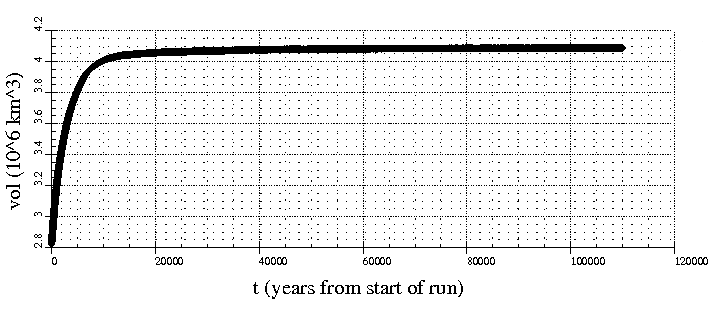
\includegraphics[width=6.0in,keepaspectratio=true]{eisgrn-volseries}
\caption{Volume time series for a 110k model year EISMINT-Greenland SSL2 run; units of $10^{6}\,\text{km}^3$.}
\label{fig:eisgrnvolseries}
\end{figure}

\begin{figure}[ht]
\centering
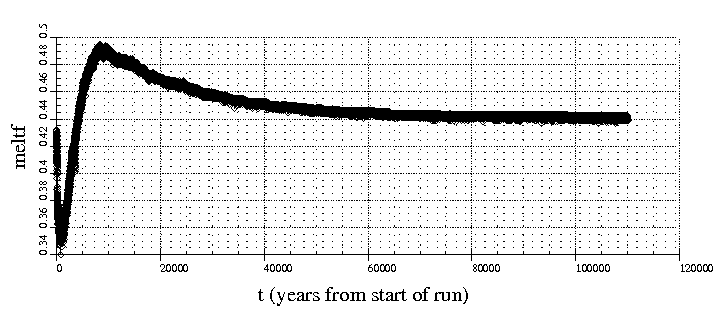
\includegraphics[width=6.0in,keepaspectratio=true]{eisgrn-meltfseries}
\caption{Time series for the fraction of the base which is at the pressure-melting temperature from a 110k model year EISMINT-Greenland run.  See the right hand part of Figure \ref{fig:ssl2thickTpa} for a map of the basal temperature.}
\label{fig:eisgrnmeltfseries}
\end{figure}

FIXME:  FIGURES NEED MAINTENANCE.   We will use the final NetCDF file \verb|green_ssl2_110ka.nc| to continue the EISMINT-Greenland experiments below.  The saved ice thickness, basal temperature, and vertically-averaged horizontal velocity maps are shown in Figure \ref{fig:ssl2thickTpa}.

\begin{figure}[ht]
\centering
\mbox{\phantom{|}\hspace{-1.0in}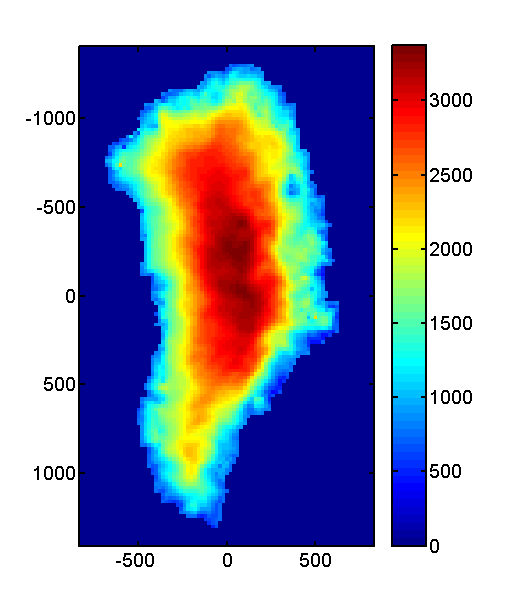
\includegraphics[height=3.0in,keepaspectratio=true]{greenH-SSL2}\,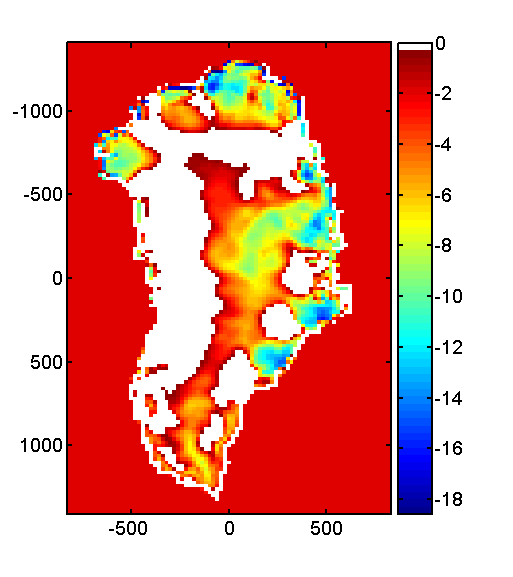
\includegraphics[height=3.0in,width=2.3in]{greenTpa-SSL2}\,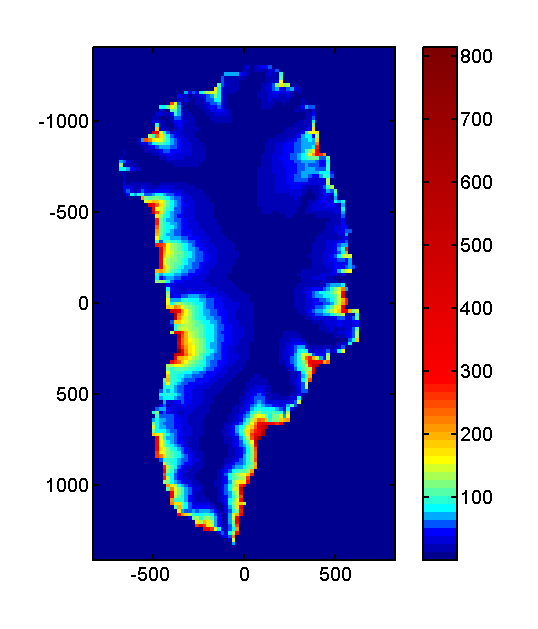
\includegraphics[height=3.0in,keepaspectratio=true]{greencbar-SSL2}}
%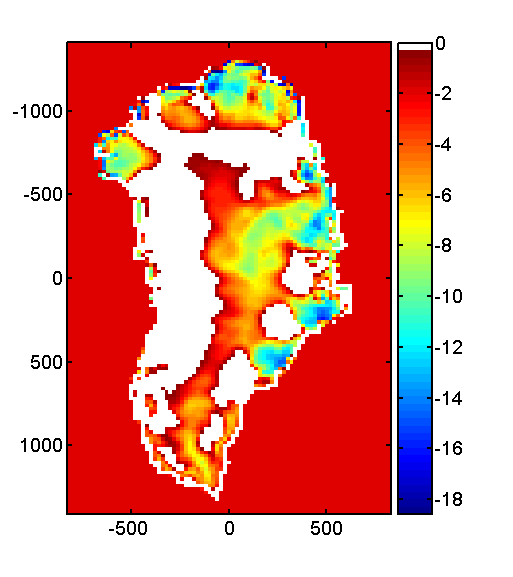
\includegraphics[height=3.7in,width=2.9in]{greenTpa-SSL2}
\caption{Ice thickness (meters; left), basal temperature (degrees C below 0; middle), and vertically-averaged horizontal velocity (m/a; right) at the end (110k model years) of a EISMINT-Greenland SSL2 run.  Note that in the temperature graph the pressure-melting temperature areas are white.}
\label{fig:ssl2thickTpa}
\end{figure}

In addition to the more standardized EISMINT-Greenland intercomparison called ``SSL2'', a ``SSL3'' was proposed to allow each participant to choose additional parameters and adjust other aspects of the model.  (Sliding, for instance, is an outstanding omission here.)  We omit this run for tutorial purposes, however, and proceed to use climate forcing in runs ``CCL3'' and ``GWL3''.


\subsubsection*{Climate forcing from GRIP and SPECMAP} 
\label{sec:climate-forcing}
The next experiment starts from the end of the steady state SSL2 run above.  Recall that the NetCDF files \verb|grip_dT.nc| and \verb|specmap_dSL.nc| contain time series data for change in surface temperature and sea level.  The options \verb|-dTforcing| and \verb|-dSLforcing| include these data for a ``CCL3'' climate forced run \cite{RitzEISMINT,HuybrechtsEISMINT}.  Before every time step, \verb|pgrn| reads the change to the surface temperature and sea level for that time.  The data in \verb|grip_dT.nc| extends 250,000 years into the past, while the data in \verb|specmap_dSL.nc| goes back about 780,000 years, so EISMINT-Greenland specifies that the run will start at the beginning of the GRIP data.  

The script \texttt{ccl3.sh} runs the CCL3 experiment for the full 250ka period, with this single command
\begin{verbatim}
mpiexec -n 8 pgrn -ccl3 -skip 10 -i green_ssl2_110ka.nc -ys -249900 -ye 0 \
  -dTforcing grip_dT.nc -dSLforcing specmap_dSL.nc \
  -save_file snaps_ccl3.nc -save_times -240000:10000:-10000 \
  -ts_file vol_ccl3.nc -ts_vars ivol -ts_times -249800:100:0 -o green_ccl3_year0.nc
\end{verbatim}
\noindent Option \intextoption{ccl3} also turns on the Lingle and Clark \cite{BLKfastearth,LingleClark} two layer, flat earth bed deformation model with an assumption of zero uplift rate at the start of the run.

FIXME:  FIGURES NEED MAINTENANCE.   The resulting thickness difference, relative to the end of the SSL2 run, and the pressure-adjusted basal temperature, are shown in Figure \ref{fig:cclthickTpa}.

\begin{figure}[ht]
\centering
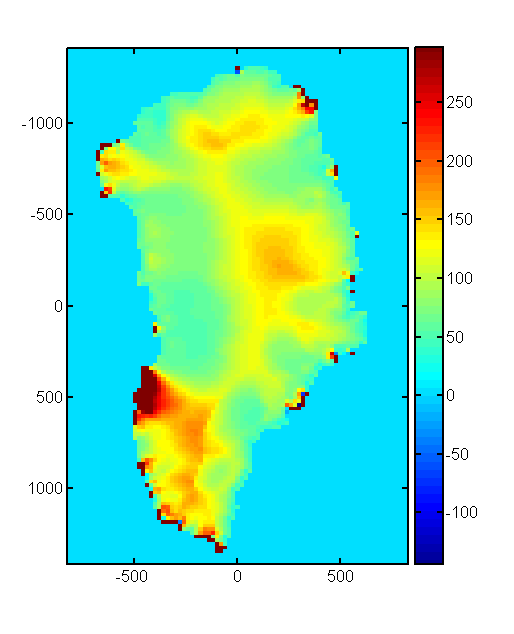
\includegraphics[width=2.8in]{Hdiff-CCLSSL}\quad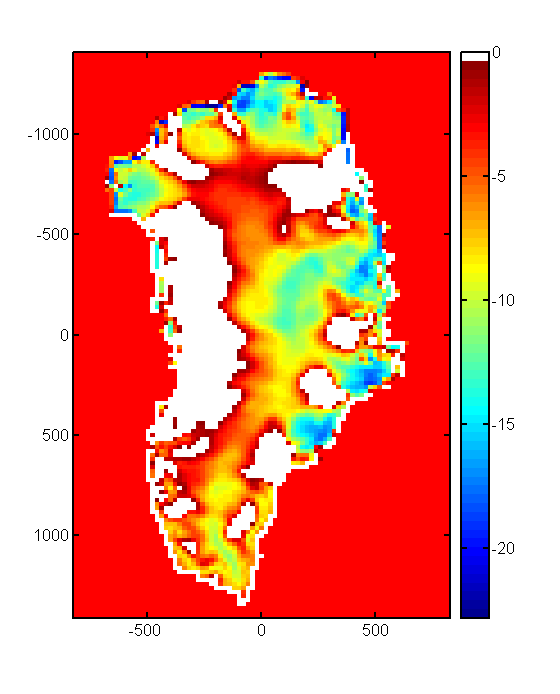
\includegraphics[width=2.8in]{Tpa-CCL}
\caption{Left:  Ice thickness difference between end (year zero) of a CCL3 run and the end of an SSL2 run (meters).  Right:  Ice pressure-adjusted basal temperature (degrees C below 0; right) at the end of a EISMINT-Greenland CCL3 run.  Compare Figure \ref{fig:ssl2thickTpa}.}
\label{fig:cclthickTpa}
\end{figure}

EISMINT-Greenland also calls for a baseline run for another 500 years which starts from the end of the CCL3 run and has steady current climate forcing (noting no GRIP or SPECMAP data are known from the future!):

\verb|mpiexec -n 8 pgrn -ccl3 -i green_ccl3_year0.nc -y 500 -o green_ccl3_year500.nc|

A final ``greenhouse warming'' experiment ``GWL3'' (options \intextoption{gwl3} and \intextoption{gwl3_start_year}) is described in the EISMINT-Greenland \cite{RitzEISMINT}.  It runs for 500 years with the temperature increasing by $0.035^\circ C/$year for the first 80 years, then at a rate of $0.0017^\circ C/$year for the last 420 years:

\verb|mpiexec -n 8 pgrn -gwl3 -i green_ccl3_year0.nc -y 500 -o green_gwl3_year500.nc|

\subsubsection*{Visualizing the climate inputs in the Greenland case}
\label{sec:pdd-series-with-pclimate}

Assuming that \verb|green20km_y1.nc| was produced by the run above (see section
\ref{sect:green-bootstrapping}), one can run the following to check if the PDD
model in PISM (see section \ref{sec:boundary-models}) is ``reasonable'':
\begin{verbatim}
$ pclimate -i green20km_y1.nc -sma -ys 0.0 -ye 2.5 -dt 0.1 -o pddmovie.nc
\end{verbatim}
This produces the file \verb|pddmovie.nc| with four variables: \verb|acab|
(instantaneous net ice equivalent accumulation (ablation) rate), \verb|artm|
(mean annual temperature at ice surface but below firn), \verb|snowtemp|
(instantaneous snow temperature) and \verb|snowprecip| (mean annual
ice-equivalent snow accumulation rate).

Variables \verb|artm| and \verb|snowprecip| do not evolve over time because the 
former is generated from ice sheet geometry and latitude by the EISMINT-Greenland
formulas \cite{RitzEISMINT}, while the latter is part of the EISMINT-Greenland data
itself.

The other two variables were used to create figure \ref{fig:pddseries}, which
shows the time-series of the accumulation rate (top graph) and the snow
temperature (bottom graph) with the map view of the snow temperature at time 0
over it. The cross on the latter shows (approximately) the location of the
point used for the time-series.

Here are two things to notice:
\begin{enumerate}
\item The summer peak day is in the right place.  The default for this value is
  August 1 (day $243$, at approximately $243/365 \simeq 0.66$ year).  (If it is
  important, the peak day can be changed using the \texttt{-pdd_summer_peak_day}
  option; subsection \ref{sec:boundary-models}).

\item Lows of the surface mass balance rate \verb|acab| correspond to 
  positive degree-days in the given period, because of highs of the snow 
  temperature.  Recall the snow temperature graph does
  not show random daily variations.  Even though it has the maximum of about $266$
  Kelvin, the parameterized instantaneous snow temperature can be above freezing.
  A positive value for positive degree-days is expected \cite{CalovGreve05}.
\end{enumerate}

\begin{figure}[ht]
  \centering
  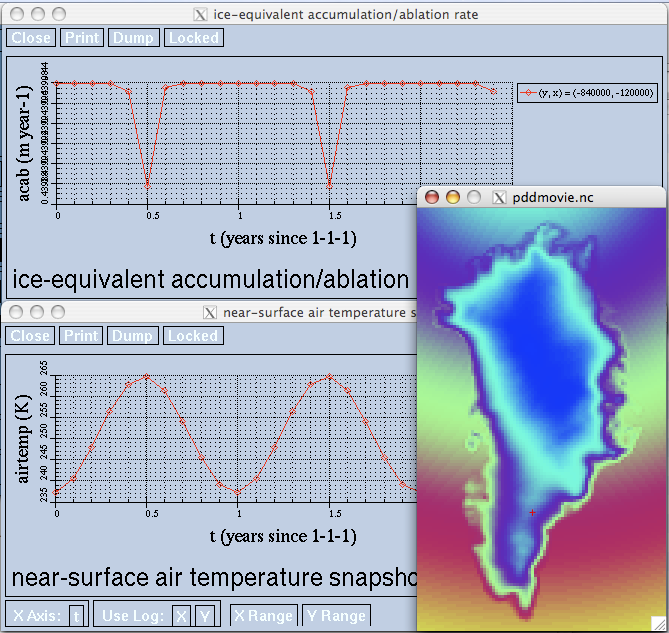
\includegraphics[width=5in]{pdd-timeseries}
  \caption{Time series of the surface mass balance rate and snow temperature. Map view 
           on the right shows the location chosen.}
  \label{fig:pddseries}
\end{figure}

\bigskip
We can also test the surface temperature forcing code with the following command.
\begin{verbatim}
$ pclimate -ca -i green20km_y1.nc -o dT_movie.nc \
          -ys -2.5e5 -ye 0 -dt 2000 -dTforcing grip_dT.nc
\end{verbatim}
The output \verb|dT_movie.nc| and \verb|grip_dT.nc| mentioned in section above were used to create figure \ref{fig:artm-timeseries}.

This figure shows the GRIP temperature offsets (top graph; compare to figure \ref{fig:gripDeltaT}) and the time-series of the temperature at the ice surface at a point in southern Greenland (bottom graph), confirming that the temperature offsets are used correctly.

\begin{figure}[ht]
  \centering
  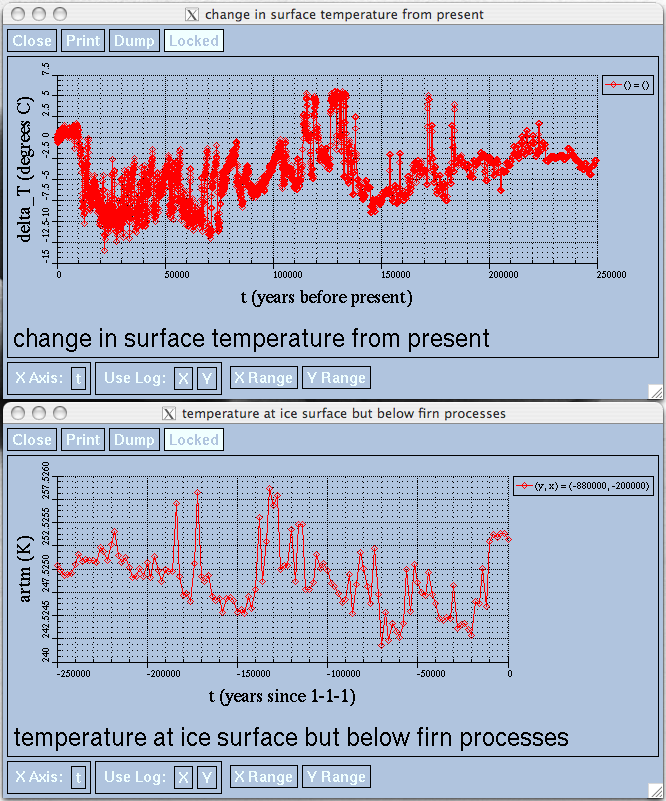
\includegraphics[width=5in]{artm-timeseries}
  \caption{Time series of the surface temperature compared to GRIP temperature offsets}
  \label{fig:artm-timeseries}
\end{figure}

FIXME:  Variable acab in following is worth looking at.  It looks right and it may be possible to compare to other paleo-limate studies:
\begin{verbatim}
$ pclimate -i green20km_y1.nc -o bar.nc -ys -125000.0 -ye -0.0 -dt 1000.0  -dTforcing grip_dT.nc -dSLforcing specmap_dSL.nc -sma
\end{verbatim}


%%% Local Variables: 
%%% mode: latex
%%% TeX-master: "manual"
%%% End: 
